\section{Vue détaillée de la démarche}
\label{sec:S1}

La figure~\ref{fig:demarche-detail} détaille la démarche résumée à la figure~1 du manuscrit. Pour chacun des trois blocs, elle précise les données d'entrée, les traitements et les sorties : la génération des crises étiquetées et de leurs quatre versions (simuler), l'ajustement de la courbe de résilience et le calcul des indicateurs (mesurer), puis l'apprentissage du réseau bayésien causal et ses trois usages (apprendre). Des vignettes illustrent une trajectoire, une courbe ajustée et la structure du réseau appris.

\begin{center}\begin{minipage}{\textwidth}\centering
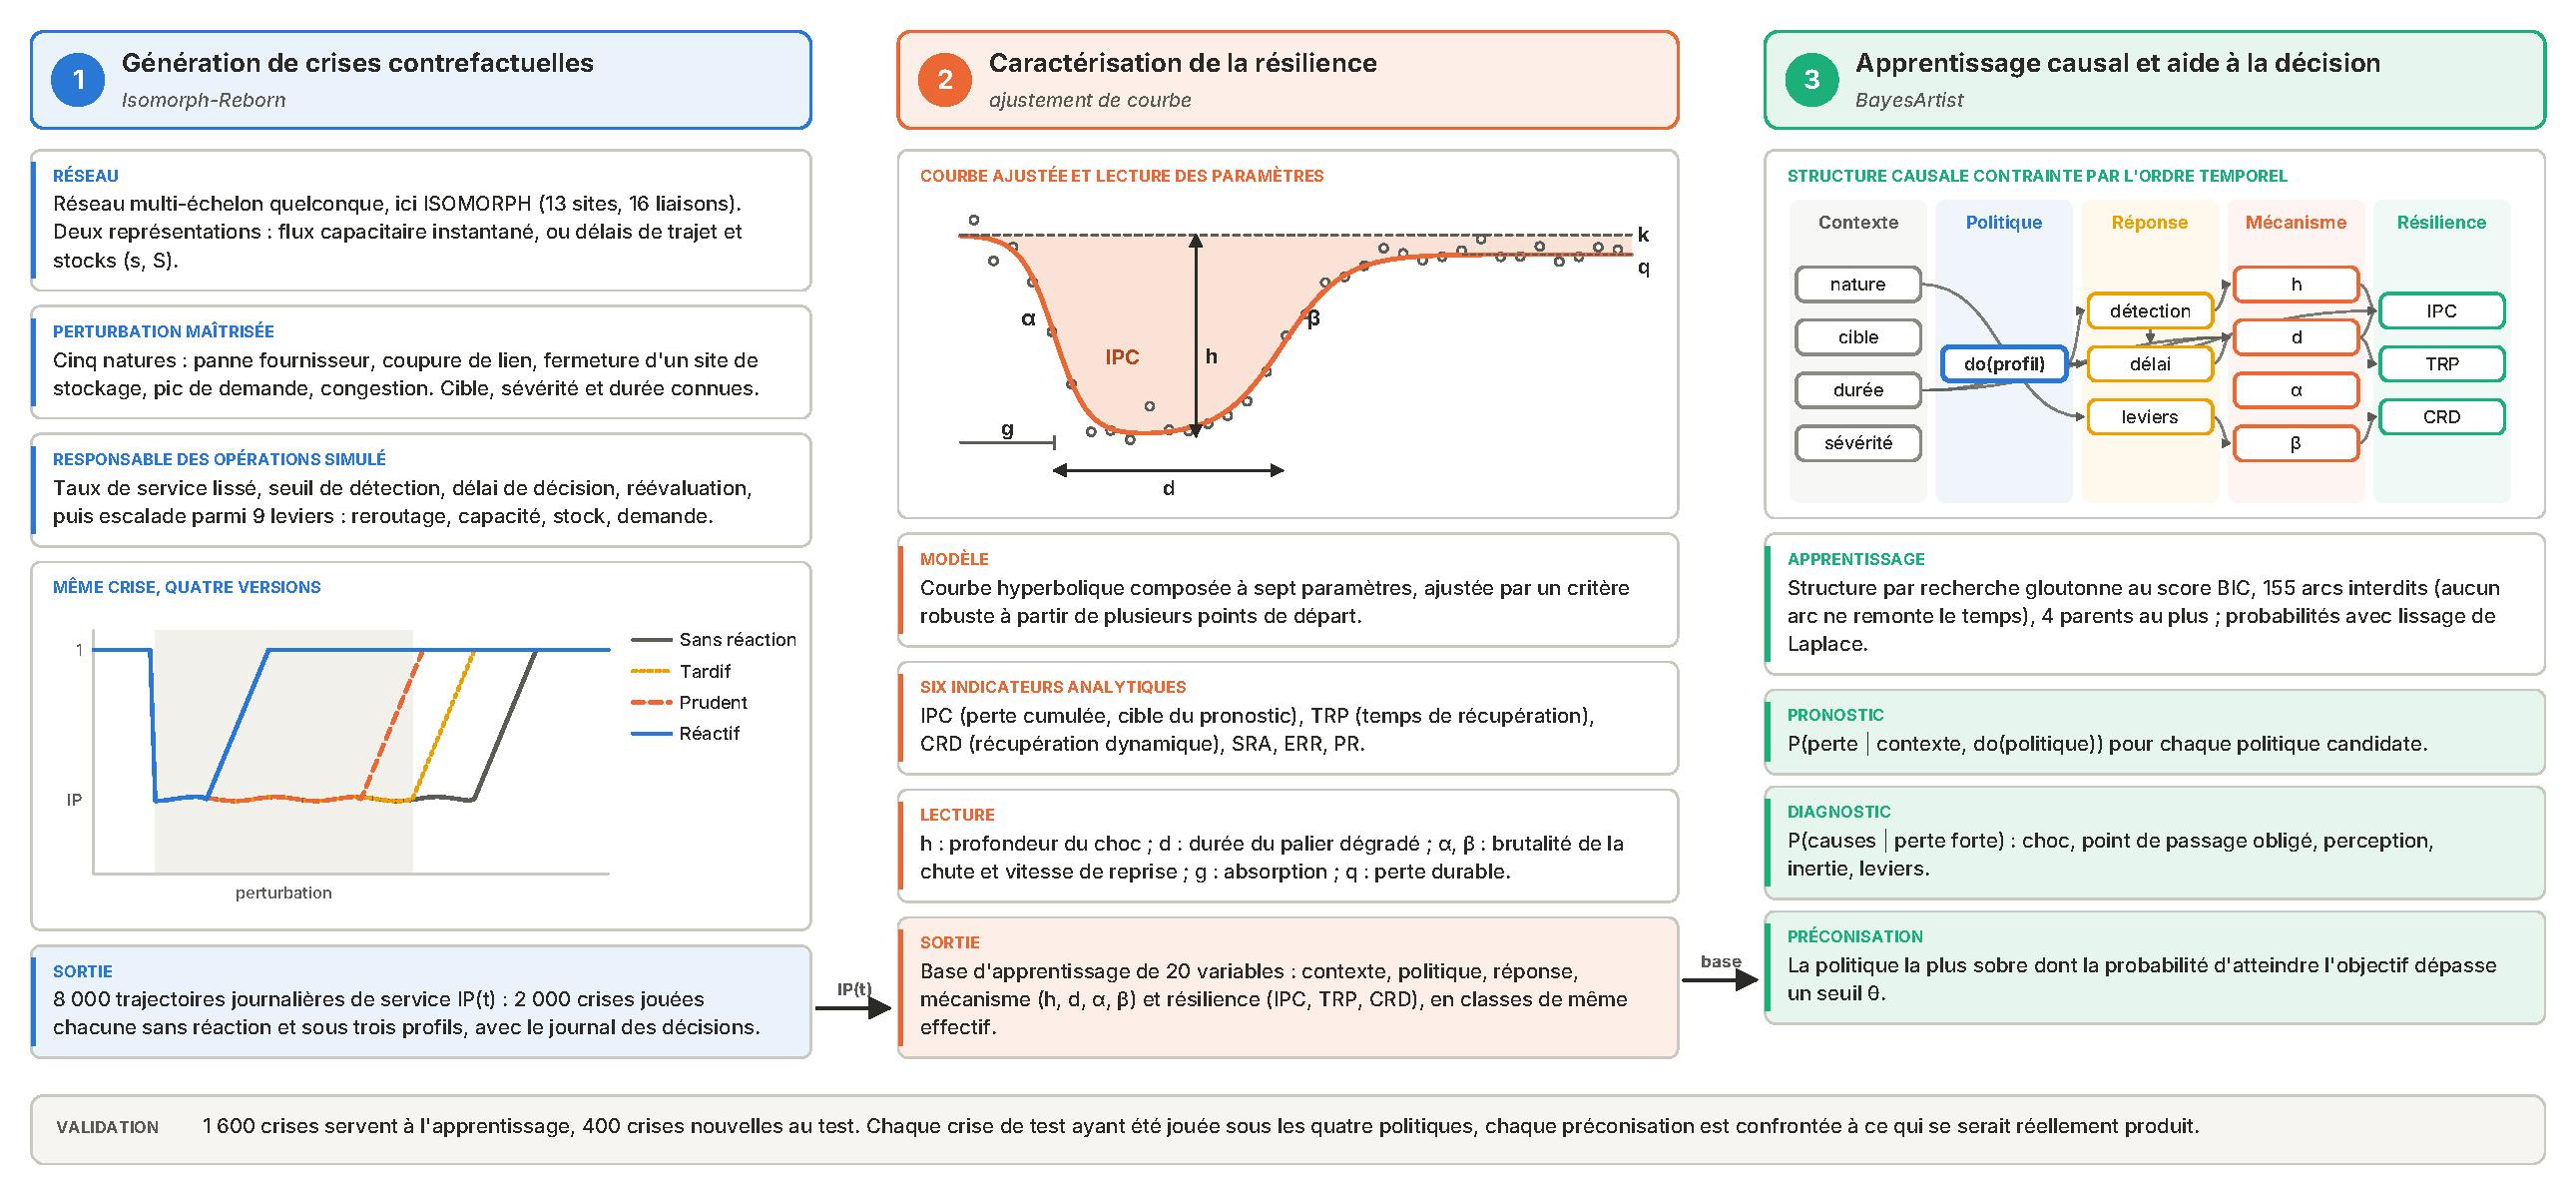
\includegraphics[width=\textwidth]{figures/Fig1_demarche.pdf}
\captionof{figure}{Démarche détaillée en trois blocs : entrées, traitements et sorties de chaque bloc.}\label{fig:demarche-detail}
\end{minipage}\end{center}
